\documentclass[openany]{book}
\usepackage[utf8]{inputenc}
\usepackage[english,brazilian]{babel}
\usepackage[editing]{coop-writing}
\usepackage[backend=biber,style=authoryear,
natbib]{biblatex}
\usepackage{graphicx} % includegraphics
\usepackage{csquotes} %enquote, textquote...
\usepackage{enumitem} % noitemsep, nolistsep
\usepackage[ruled,vlined,portuguese,linesnumbered]{algorithm2e}
\usepackage[scale=5]{ccicons}
\usepackage{indentfirst }
\usepackage{draftwatermark}
\SetWatermarkText{DRAFT}
\SetWatermarkScale{1}
\setlist[itemize]{noitemsep}
\setlist[itemize]{nolistsep}
\setlist[enumerate]{noitemsep}
\setlist[enumerate]{nolistsep}

\renewcommand*{\mkcitation}[1]{ #1}
\usepackage{outlines}

\addbibresource{ec.bib}

\cwnamedef{xexeo}{red}{Xexéo}
\setlength{\parskip}{0.5em}
\setlength{\cftsubjectnumwidth}{20pt}
\setlength{\cftcomentarionumwidth}{20pt}
\setlength{\cftcomentariorefnumwidth}{20pt}
\usepackage{titling} % construir página de title
\title{Dicas de Escrita de Artigos Científicos}
\author{Geraldo Xexéo}
\date{\today}
\predate{\centering}
\postdate{\vfill\hfill\ccbyncsa\hfill}


\begin{document}

\frontmatter

\maketitle

\tableofcontents



\chapter*{Licença}

\begin{center}
\ccbyncsa

\vspace{1cm}

Este texto é distribuído com uma licença Creative Commons - Atribuição - NãoComercial - CompartilhaIgual 4.0 Internacional.

\end{center}






\section*{Você tem o direito de:}
\begin{itemize}
\item \textbf{Compartilhar} -- copiar e distribuir o material em qualquer suporte ou formato.
\item \textbf{Adaptar} -- remixar, transformar, e criar a partir do material.
\end{itemize}

\section*{De acordo com os termos seguintes:}
\begin{itemize}
\item \textbf{Atribuição} -- Você deve dar o crédito apropriado, prover um link para a licença e indicar se mudanças foram feitas. Você deve fazê-lo em qualquer circunstância razoável, mas de nenhuma maneira que sugira que o licenciante apoia você ou o seu uso.
\item \textbf{NãoComercial} --Você não pode usar o material para fins comerciais.
\item \textbf{CompartilhaIgual} -- Se você remixar, transformar, ou criar a partir do material, tem de distribuir as suas contribuições sob a mesma licença que o original.
\item \textbf{Sem restrições adicionais} -- Você não pode aplicar termos jurídicos ou medidas de caráter tecnológico que restrinjam legalmente outros de fazerem algo que a licença permita.
\end{itemize}

Mais informações podem ser encontradas em \url{https://creativecommons.org/licenses/by-nc-sa/4.0/deed.pt_BR}

\mainmatter

\chapter{Introdução}
\cwmain{Este texto apresenta dicas de escrita de artigos científicos, em especial para Computação, com foco em brasileiros que tem que escrever em inglês.} Essas dicas foram coletadas a partir da leitura de vários livros, artigos e sites que serão indicados ao longo do texto.

O fato de eu escrever este documento não significa que eu escreva bem, mas que eu me esforço para isso e que, com o tempo, adquiri um conhecimento que me permite, principalmente, criticar o meu próprio trabalho e o dos outros como revisor.

As dicas aqui colocadas tem esse objetivo específico e, em geral, não são perfeitamente adequadas para outras formas de escrita.

\cwmain{Este texto está sendo distribuído com o pacote \texttt{coop-writing}, onde coloquei marquei com o comando \texttt{cwmain} os inícios de parágrafos para demonstrara técnica de construí-los a partir de uma ideia única que os inicia.} Algumas vezes, não consegui achar a melhor forma de fazer isso, outras vezes, como nas regras e dicas mais diretas, isso não é possível.

\section{Não é fácil escrever}

\cwmain{Escrever não é fácil.} Um iniciante pode acreditar que textos são escritos uma vez e estão prontos. Não é verdade. Textos de qualidade foram escritos e reescritos, revisados e editados.

\cwmain{É necessário reescrever e revisar muitas vezes um texto para que fique bom}, e nem cito a palavra ótimo\footnote{Como diz o ditado popular ``O ótimo é inimigo do bom''. A interpretação correta desse ditado é que se tentamos ser ótimos podemos não conseguir ser bons.}, para ser aceito por uma revista ou congresso científico. Reescrevemos o texto para ele ficar mais claro e  compreensível. Revisamos o texto para ele ficar correto ortográfica, gramática e estilisticamente.

\cwmain{Escrever em uma segunda língua, como é para nós o inglês, é ainda mais difícil.} Principalmente para quem não viveu por um tempo razoável falando em inglês diariamente. Temos dificuldade com as palavras mais adequadas, com as estruturas e com a forma de expressar nosso pensamento que vão muito além daquelas que enfrentamos em inglês.

\cwmain{Para diminuir a dificuldade de escrever em inglês é \textbf{importante ler em inglês}.} Isso trará justamente o conhecimento da ortografia, da gramática e do estilo adequado. Se o escritor não lê na língua que escreve, não tem uma base de exemplos suficiente para poder criar o seu texto.

\cwmain{A dica principal para escrever é \textbf{comece a escrever}}. É muito mais fácil corrigir do que iniciar um texto, assim, se você já tem algum texto escrito, ou uma lista de itens a preencher, fica mais fácil. A técnica básica é criar lacunas para serem preenchidas.

\cwmain{Iniciar a escrever leva a outra técnicas: planeje seu texto}. É importante ter uma estrutura e um guia do que você deve fazer para saber não só o que vai fazer, mas também o que não vai. Parte de qualquer plano é dizer onde certas coisas são feitas e onde certas coisas não são feitas. Assim, com uma estratégia de dividir para conquistar, você atinge mais facilmente seu objetivo.


\chapter{Estilo}

\section{O que é estilo de escrita?}

\cwmain{Um estilo de escrita é uma forma de expressar as ideias através de texto.} Um texto é composto de palavras ordenadas em uma sequência específica, e possui um significado. Se você se lembra do seu curso fundamental e médio sabe que existe a ortografia e a gramática, que falam das palavras e da estrutura do texto. Além disso, temos o significado, ou semântica. Também temos a pragmática, que analisa o texto dentro de um contexto. Mais além, temos um efeito da forma como as ideias são apresentadas, como as palavras e estruturas são escolhidas, talvez fortemente estético, que agrada mais, ou menos, seus leitores, ou torna mais fácil, ou mais difícil, a leitura. Essa forma é o estilo.

\cwmain{O estilo de escrita pode ser analisado de várias formas}, como em relação a um escritor, como o estilo de escrita de José Saramago, como em função de uma nacionalidade ou época, o estilo da poesia barroca brasileira, etc. Uma das formas é em função do objetivo geral do texto, como informar, descrever, etc., caracterizando um tipo de estilo. Na escrita científica, existe um estilo geral, mas revistas e congressos também tem estilos próprios.

\cwmain{Alguns tipos de estilo reconhecidos são o expositivo, o descritivo, o persuasivo e o narrativo}\citep{jeffrey:2016}. Esses tipos de estilo possuem características próprias, sendo o expositivo o mais comum em artigos científicos. Porém, pelos nomes, é possivel ver que um mesmo texto pode apresentar mais de um desses estilos. A revisão bibliográfica de um artigo, por exemplo, pode ser mais descritiva ou expositiva, já a  conclusão  pode ser mais persuasiva.

\cwmain{Para escolher um estilo de escrita é necessário conhecer o seu objetivo e quem são os seus leitores.} A audiência tem expectativas que devem ser atendidas, e, quando quebradas, podem deixar o leitor desconcertado e evitar que eles leiam seu artigo.

Como é importante conhecer esses leitores, é muito útil, também, \cwmain{saber em qual veículo, revista ou congresso, o artigo será publicado.}

\cwmain{Existem regras, ou pelo menos padrões, tradicionais de estilo em escrita científica de artigos em inglês.} Por exemplo, devemos evitar  a voz passiva.

\cwmain{Só podemos quebrar essas regras se sabemos muito bem o que estamos fazendo.}
Bons autores tem estilo próprio que quebram algumas regras, ou mesmo todas, porém devemos considerar duas coisas: primeiro, não estamos fazendo literatura, segundo, se você está lendo esse texto, provavelmente ainda não chegou no nível de experimentar com os estilos.

\cwmain{Alguns autores procuram formas excessivamente complicadas de se expressar em artigos científicos}. As sentenças na lista a seguir usam estilos diferentes para passar a mesma ideia geral. Eu exagerei ao criar esses exemplos, mas é a sensação que tenho ao ler alguns artigos.
\begin{itemize}
    \item Foi necessário, por mim, convocar o competente discente João para auxiliar a remover mais rapidamente os entraves que obstaculavam a sua inscrição nesse instituto educacional.
    \item João, um valoroso aulista, foi convocado por mim para deslindar alguns empecilhos para sua matrícula.
    \item Chamei João, que é um bom aluno, para resolver problemas com sua matrícula.
\end{itemize}



\cwmain{Devemos procurar um estilo que facilite a leitura.} Para mim, isso significa, entre outra coisas:
\begin{itemize}
    \item usar inglês simples, com palavras que não precisam ser buscadas em um dicionário;
    \item limpar as sentenças de advérbios e adjetivos que são julgamento de valor e não podem ser comprovados, como em ``algoritmos de redes neurais têm desempenho excepcional'';
    \item construções diretas das sentenças, que não devem ser longas ou cheias de vírgulas, e
    \item evitar jargões, principalmente de outras áreas que não a tratada no artigo.
\end{itemize}

 \cwmain{Eu gosto, por exemplo, da ideia de usar listas explícitas.}
 É um estilo pessoal, e não é um inglês muito rico, porém elas facilitam a visualização de ideias e exemplos, sendo muito melhores para isso do que colocar dois pontos e seguir com uma lista de itens separados por vírgulas.

  \cwmain{Essas listas podem ser transformadas facilmente em parágrafos ou incluídas dentro de um texto, seguindo o dois pontos.} Por exemplo, se cada item da lista precisar de uma explicação, é possível transformá-los em parágrafos distinto, com palavras de ligação entre os parágrafos como ``First'', e ``Second''. O segundo caso pode ser necessário se falta espaço no artigo.

\section{A distância entre o que escrevemos e o que é compreendido}

\cwmain{Existe uma distância muito grande entre o que pensamos e o que vai entender o leitor de nosso texto.} Essa distância pode levar a compreensão errada de nossas ideias.

\cwmain{Como podemos ver pelos exemplos anteriores, a mesma ideia pode ser passada, corretamente, por vários textos.} Do mesmo modo, o mesmo texto pode gerar várias ideias.

\cwmain{A frase ``Vi um homem de binóculos'' mostra como um texto pode ser lido de várias formas.}
Ela permite duas interpretações: eu estava usando um binóculo, ou o homem portava um binóculo. Ela pode ser reescrita de outras formas para evitar essa ambiguidade, por exemplo: \enquote{De binóculo, vi um homem}, \enquote{Eu usava um binóculo quando vi um homem a distância}. Todas essas frases estão corretas, mas a original é totalmente ambígua\footnote{A ambiguidade, nesse caso, é gramatical, já que duas estruturas gramaticais podem ser construídas}, não nos permite afirmar, com certeza, se quem estava de binóculo era eu, ou o homem. A segunda, dependendo de onde é usada, poderia ainda dizer que quem estava usando o binóculo era o homem, por exemplo se respondendo a questão ``Você viu alguém com binóculo ou chapéu?''.
Na terceira tudo está mais claro e é difícil escolher um contexto onde não represente exatamente o fato de que eu estava de binóculo e não o homem.

% need to protect references in a box to allow
% highlighting
\cwmain{A Figura {\ref{fig:tr1}} ilustra a distância entre o que pensamos e o que o leitor vai interpretar} quando obtém um documento por meio de um mecanismo de busca.

\begin{figure}
    \centering
    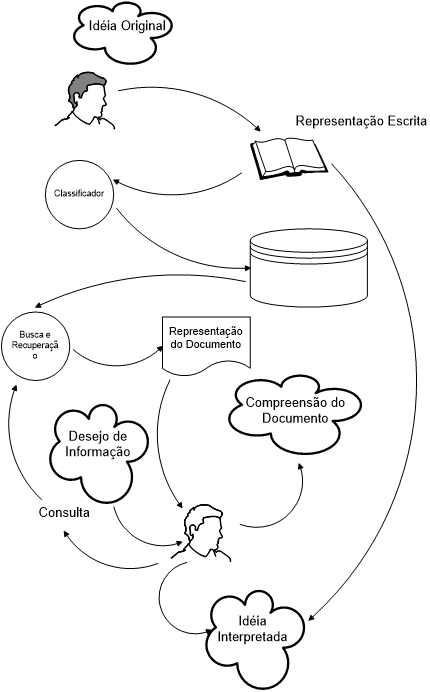
\includegraphics[height=12cm]{imagens/textretrieval.png}
    \caption{Da ideia do autor a ideia do leitor, muito pode acontecer. (desenho do autor)}
    \label{fig:tr1}
\end{figure}

\section{O problema de múltiplos autores}

\cwmain{Em um artigo de vários autores, eles devem se organizar em torno de um estilo único.} Uma das dificuldades de escrever artigos em co-autoria é normalmente a mistura de estilos. Escolhendo, ou mesmo se submetendo a um estilo único, os autores evitam que o leitor tenha a sensação de estar lendo uma colagem ou colcha de retalhos.

\chapter{O Texto Científico}

\section{O objetivo do texto científico}

\cwmain{O objetivo do texto científico é passar uma ideia complexa de forma compreensível para uma audiência internacional, onde a maioria sabe o inglês como segunda língua}. Essa ideia deve adicionar algo ao corpo de conhecimento de uma área de pesquisa.

\cwmain{A norma, então, deveria ser escrever textos simples.} Entretanto, cada revista ou congresso costuma adotar um estilo diferente, muitas vezes  rebuscado ou que exige forte conhecimento de notações e jargões pré-estabelecidos.

Minha hierarquia de objetivos é a seguinte:
\begin{enumerate}
    \item Divulgar minha pesquisa ou proposta;
    \item Permitir que sejam facilmente compreendidas;
    \item Facilitar ao leitor a leitura completa do artigo;
    \item Convencer o leitor que minhas propostas e opiniões estão corretas, e
    \item Atender as regras do meio de publicação.
\end{enumerate}

Para isso precisamos atingir algumas qualidades:
\begin{itemize}
    \item A \textbf{necessidade}, não colocando no texto material desnecessário. Tudo que está no texto deve ter uma finalidade.
    \item A \textbf{concisão}, usando o menor texto possível que seja adequado ao contexto.
    \item A \textbf{clareza}, não criando construções convolutas.
    \item A completude ou fechamento do texto, permitindo que o leitor, com o \textit{background} adequado, compreenda o texto.
\end{itemize}

\cwmain{ A audiência de um artigo possui um conhecimento específico que não devemos replicar no artigo.} Esse \textit{background}, permite tratar de assuntos sem que tenhamos de reconstruir a história da área, o que é desnecessário e torna o artigo aborrecido.




\chapter{O Processo de Publicação}

\cwmain{Publicar é parte importante do processo de pesquisa.} Divulgar os resultados e obter um \textit{feedback} dos pares faz parte do trabalho do pesquisador. Neste capítulo vamos fazer uma pequena revisão de como isso acontece.

\section{O processo básico}

\cwmain{O processo de publicação de um artigo para revista possui inicialmente seis passos básicos: aceitação inicial pelo editor, busca de revisores, análise dos revisores, divulgação do resultado pelo editor, correções pelo autor, aceitação final}. Possivelmente o resultado exigirá uma alteração do texto pelos autores, o que leverá o artigo a voltar a fase de análise dos revisores. Em congressos, raramente isso acontece, sendo o primeiro resultado normalmente final.

\cwmain{Mesmo após um resultado positivo de aceitação, tanto em congresso quanto em revistas, é normalmente necessário fazer pequenas correções para ter o artigo publicado}. Assim, o processo de publicação pode ser representado de forma geral em um Diagrama de Atividades UML 2.5, como o da Figura \ref{fig:processo}.


\begin{figure}
    \centering
    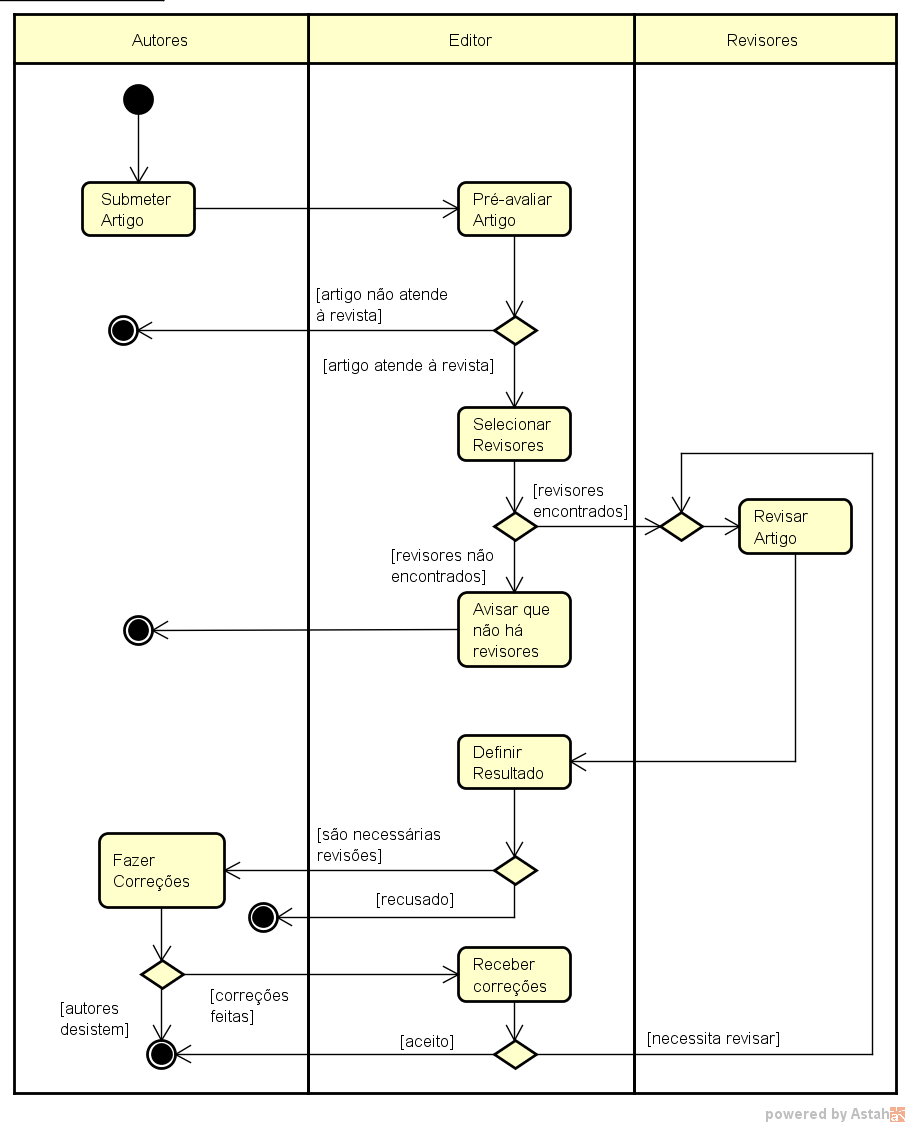
\includegraphics[width=0.7\linewidth]{imagens/ProcessoDeSubmissao.png}
    \caption[Processo genérico de submissão e aceitação de um artigo científico]{Processo genérico de submissão e aceitação de um artigo científico. (imagem do autor)}
    \label{fig:processo}
\end{figure}

\cwmain{O artigo, durante o processo, passa por alguns estados,} que podem ser representados por um Diagrama  de Estados UML 2.5 como o da Figura \ref{fig:maquina}.

\begin{figure}
    \centering
    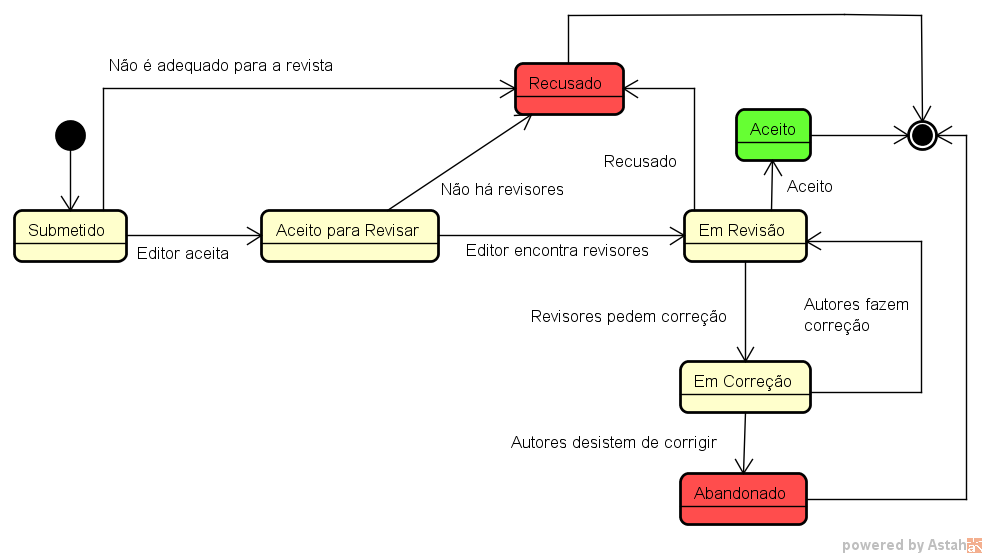
\includegraphics[width=0.7\linewidth]{imagens/MaquinaEstadoArtigo.png}
    \caption[Visão genérica dos estados de um artigo científico]{Visão genérica dos estados de um artigo científico submetido ao processo de revisão de uma revista. (imagem do autor)}
    \label{fig:maquina}
\end{figure}

\cwmain{Algumas vezes os editores não aceitam o artigo por acharam que não está no escopo da revista}. Isso indica, por um lado, que os autores não fizeram o dever de casa corretamente ao escolher a revista. Por outro lado, o editor pode sugerir revistas mais adequadas, pela especialização, pelo estilo do texto, ou por outro motivo.


\cwmain{Existe a possibilidade do artigo não ser aceito porque não foram achados revisores.} Isso já aconteceu comigo com o mesmo artigo em duas revistas, porque misturamos assuntos demais em uma tese de doutorado. Nesse caso, a solução foi buscar uma reescrita que aborde apenas um subconjunto dos assuntos. Em geral, é possível pesquisar melhor por uma revista mais adequada.

\cwmain{Processos de submissão podem se transformar em ciclos razoavelmente longos.} Isso acontece tanto porque os passos são muito longos no tempo, provavelmente devido ao atraso dos revisores, para os quais existem muitas causas, quanto porque o ciclo de revisão e correção pode acontecer mais de uma vez.

\cwmain{As revisões geralmente são classificadas em \textit{minor revision} ou \textit{major revision}}. Como o nome indica, uma \textit{major revision} indica que o trabalho de correção do artigo será grande, muitas vezes envolvendo o próprio experimento. Já uma \textit{minor revision} normalmente indica pequenos problemas de escrita. Possivelmente uma \textit{minor revision} não precisará ser revisada de novo pelos editores.

\cwmain{Uma \textit{minor revision} é praticamente uma aceitação.} Os autores devem considerar isso um ótimo sinal sobre o artigo. O muito importante não perder uma chance de publicação indicada por uma \textit{minor revision}, e isto pode acontecer principalmente por causa do prazo que foi dado.

\cwmain{Uma \textit{major revision} indica que o artigo tem alguma substância, mas ainda não atingiu o padrão da revista.} Normalmente o trabalho de uma \textit{major revision} vale a pena, mas alguns autores desistem, principalmente quando são necessárias muitas mudanças significativas na parte experimental ou o prazo para as correções é muito curto. É possível que procurem outra revista, mesmo que façam algumas das correções.

\cwmain{Raramente um artigo é aceito em sua primeira versão.} Eu diria que a probabilidade é equivalente a de um \textit{hole in one} no golfe.

\cwmain{É comum que um artigo recusado seja corrigido,  a partir dos comentários dos revisores, e submetido, inicialmente a outra revista, eventualmente a mesma}. Isso é o fluxo normal de muitos artigos, que vão sendo melhorados até serem aceitos, ou são submetidos a revistas ou congressos com chances maiores de aceitação, ou mais adequados aos tópicos de artigos.

\cwmain{É importante não se sentir desanimado com uma recusa}. O processo de revisão por pares é um processo de aprendizado e raramente a crítica é errada.


\cwmain{É possível que o resultado final seja \textit{Revise and Resubmit}}. Isso é mais parecido com uma recusa, porém o editor acha que o artigo, se corrigido, normalmente de forma drástica, cabe na revista, porém todo o processo vai ser refeito do início. Essa resposta não está retratada nas figuras por ser basicamente uma recusa educada.

\subsection{Galley Proofs}

Algumas editoras tem o hábito de usar \textit{galley proofs}. Isso significa que elas enviam para você uma versão final do texto como será publicado, e dão uma chance de você identificar erros, principalmente na formatação. Tradicionalmente isso acontecia porque o texto era tipografado, mas atualmente, com o uso de estilos, \LaTeX ou Word, esse passo muitas vezes não existe


\section{O que analisam os revisores}

\cwmain{Em cada conferência ou publicação os revisores são solicitados a analisar algumas características no artigos.} Essa análise é feita na forma de notas, como um valor entre um a 10, ou na forma de escolha entre uma lista de opções, como ``totalmente original'' e ``não apresenta nenhuma ideia nova''.


\cwmain{Um fator que está sempre presente é a originalidade do artigo.} A originalidade, em geral, pode variar entre algo nunca antes pensado até um resultado conhecido e trivial que foi simplesmente repetido. Devemos pensar a originalidade como uma linha contínua. Um ponto dessa linha pode ser ``Aplicar um algoritmo conhecido em um novo problema'', e outro, de melhor qualidade pode ser ``Melhorar o estado da arte de solução de um problema por meio da modificação de um algoritmo existente''. Certamente criar algoritmos que melhoram o estado da arte e provar teoremas em aberto há algum tempo estão entre as propostas mais fortes.

\cwmain{A clareza e correção do do texto também são quesitos sempre presentes}. É comum vermos um pedido para que o artigo seja revisado por um nativo da língua (inclusive para autores nativos!). Sim, nativos da língua que sabem escrever bem são poucos, e ainda por cima, espera-se um estilo semelhante ao inglês britânico ou americano\footnote{É importante manter a consistência ortográfica entre uma dessas formas. ``Color'' e ``tire'' são versões americanas das palavras britânicas ``colour'' e ``tyre''.}.

\cwmain{Outro fator muito comum é a exigência de uma base teórica sólida.}

\cwmain{Normalmente também cabe ao revisor julgar se o artigo é apropriado para a conferência ou revista.} Mesmo que o editar já tenha feito um primeiro filtro.

\section{Revisões claramente mal feitas}


\cwmain{Não é raro que uma revisão seja mal feita}. Principalmente em congressos, onde os dados mostram que há pouca concordância entre os revisores\favorcitar.

\cwmain{Alguns casos que eu conheço de revisões mal feitas}:
\begin{itemize}
    \item Um artigo foi recusado em uma trilha de uma conferência porque um revisor considerou que a trilha, de \textit{design}, era restrita a arte de jogos, e não incluia o \textit{game design};
    \item Um revisor afirmou que ``o autor não poderia ter um trabalho dessa qualidade sem nunca ter publicado na área, logo devia ser mentira''.  Essa resposta já foi vista duas vezes, em um congresso e em uma revista, por autores diferentes. No caso da revista o autor recorreu ao editor e teve o artigo publicado.
    \item Revisores que apresentaram revisões (de recusa) de outros artigos. Isso também já aconteceu mais de uma vez, infelizmente em conferências onde não era possível revisar o resultado. É culpa não só do revisor, mas também do responsável pelas revisões.
\end{itemize}

\cwmain{Se a revisão mal feita é para uma revista, não exite em contatar o editor.} Ele pode realmente tomar alguma atitude. Se é para um congresso, provavelmente não haverá muita chance de reclamar, mas é importante avisar o editor para que ele evite problemas no futuro. Provavelmente o artigo poderá ser facilmente aproveitado em outro congresso ou revista.

\cwmain{Principalmente em congressos, é possível que um artigo receba revisões muito díspares.} Eu já tive um artigo revisado por três revisores que disseram: não é da área e deve ser recusado, é um artigo limítrofe entre aceitar ou não e é um dos melhores artigos do congresso. Isso causa uma certa revolta ao autor, mas acontece muito quando o veículo de publicação é mais heterogêneo e composto de muitas áreas, e os artigos são distribuídos por sorteio aos revisores.

\section{A correção}

\cwmain{Acompanhando a correção, os autores devem enviar um documento explicando como cada pedido dos revisores foi, ou não, atendido}. Esse documento é importantíssimo para os revisores entenderem o que foi feito, e é também uma prova de que o processo de correção foi bem feito pelos autores.

\cwmain{Esta carta é mais importante se for uma \textit{major revision}}. Os itens devem ser tratados em ordem de importância, do mais importante para o menos importante, já que elas provavelmente terão uma impacto maior no artigo.

\cwmain{Tipicamente esse documento é uma lista dos pedidos feitos, onde cada item é seguido da explicação da correção feita.} Essa explicação pode ser pequena ou grande, dependendo realmente do que foi feito.

\cwmain{É importante que essa lista tenha um formato muito legível.} Afinal, o objetivo é ajudar os revisores a entender a sua correção, e não criar mais confusão.  Quando for razoável, é bom mostrar a versão anterior e a nova versão.



\section{Considerações finais sobre o processo de publicação}

Nunca espere que seu artigo seja aceito como submetido da primeira vez. Ser aceito como \textit{major revisions} por uma boa revista é uma vitória. Conseguir atender essas revistas é uma vitória ainda maior.



\chapter{Escolha da revista}

\cwmain{A escolha da revista ou conferência pode ser feito de forma estratégica em função do seu objetivo ao publicar.} Nessa escolha podem ser analisados, entre outros fatores:
\begin{itemize}
    \item a adequação ao tema e originalidade do artigo;
    \item a qualidade da publicação;
    \item o estilo dos artigos na revista;
    \item o tempo de resposta médio de revisão e aceitação;
    \item a quantidade de artigos aceitos em relação aos submetidos;
    \item a quantidade de artigos publicados por ano e por exemplar, e
    \item a experiência dos autores com a revista ou conferência.
\end{itemize}

\cwmain{Devemos publicar na revista ou congresso mais adequados ao tema do artigo.} Existem algumas complicadores para isso. Em áreas novas de pesquisa, pode ser que nenhuma publicação específica tenha uma reputação que atenda a próxima questão, a qualidade da publicação. Também é possível que as revistas que parecem mais adequadas possuam processos muito longos, algumas possuem processos de mais de um ano, que não atendem a necessidade de um dos autores. Na COPPE, por exemplo, é preciso publicar em uma revista indexada para defender a tese de doutorado, mas claramente o candidato ao doutorado não pode se arriscar a esperar anos pela aceitação.

\cwmain{A qualidade da publicação depende de vários fatores.} Existem fatores subjetivos, como a reputação da revista na comunidade, e fatores objetivos, como índices bibliométricos, como o índice JCR ou o índice H. Algumas áreas, que possuem menos pesquisadores ou são bem específicas, por exemplo, tem indicadores objetivos bem baixos, porém as suas revistas tem grande reputação. Nessa questão, os orientadores podem ajudar muito os alunos autores.

\cwmain{Quanto ao estilo, algumas revistas exigem uma abordagem muito formal, enquanto outras aceitam uma linguagem mais informal.}. Por exemplo, para alguns autores é difícil reescrever um trabalho que foi feito de forma mais prática, com algoritmos e programas, na forma de equações matemáticas. Isso pode evitar que um artigo seja adequado a um grupo de revistas que são fortemente baseadas em matemática. Para ilustrar, o texto, a fórmula e o algoritmo a seguir apresentam dois estilos de dizer  a mesma coisa: a média aritmética de um conjunto de valores é a soma dos valores dividida pela quantidade de valores.

% TIL: \limits faz os limites inferior e superior
% ficarem abaixo e acima do símbolo de somatório.
\begin{equation}
    \bar{x} = \frac{\sum\limits_{i=1}^{N}x_i}{N}
\end{equation}

\begin{algorithm}
    \KwIn{$X=\{x_i | 1<i\leq N\}$}
    $S \leftarrow 0$ \;
    $K \leftarrow |X|$ \;
    \While{$|X|>0$}{
        $S \leftarrow S + x_1$\;
        $X \leftarrow X - \{x_1\}$\;
    }
    \Return{$S/K$}
    \caption{Média Aritmética}
\end{algorithm}

\section{Índices bibliográficos objetivos}

\todo[inline]{Explicar JCR, H e como achar esses números. Falar sobre as indexações importantes e as que são apenas mecanismos de busca}

\cwmain{Os índices objetivos das revistas ajudam a tomar decisões práticas.} Nem toda revista oferece esses dados, mas as que oferecem permitem que os autores analisem se é prático publicar nas mesmas. Uma revista com um processo muito lento é inadequada para quem tem prazo ou pressa. Porém, a qualidade da publicação deve ser sempre levada em conta. Esperar mais um pouco por uma publicação bem melhor pode causar uma grande modificação no impacto do artigo na área.

\section{O que é uma boa revista}

Uma boa revista tem reputação na área, e isso se aprende com o tempo. Uma revista muito citada, normalmente é uma boa revista.

No Brasil, temos uma classificação de qualidade de revistas conhecida como Qualis. Ele apresenta vários defeitos, mas o que eu considero principal é o fato de algumas áreas considerarem muitas publicações nacionais, sem impacto internacional, como de ótima qualidade.

O Qualis classica as revistas em três níveis, subdivididos em estratos\footnote{Aqui se descreve o que é conhecido no ``novo Qualis''}. Os níveis são A, B e C; e ainda existe o NP.  Cada nível é dividido em estratos, onde 1 é o melhor estrato. Os níveis A e B são divididos de 1 a 4. Uma revista no nível A é certamente uma ótima revista. O nível C não tem subdivisão.


\chapter{Inícios Devem Ser Fortes}

\cwmain{Devido a uma ideia, que considero errônea, que a introdução deve partir de algo muito geral, muitos autores começam seu artigo com um texto que não traz nenhuma informação nova}, logo não atiça a curiosidade do leitor, nem o prepara para o que está por vir.

\citeauthor{Knuth:1997} dizem:

\textquote[{\citep{Knuth:1997}}]{The opening paragraph should be your best paragraph, and its first sentence should
be your best sentence. If a paper starts badly, the reader will wince and be resigned to
a difficult job of fighting with your prose. Conversely, if the beginning flows smoothly,
the reader will be hooked and won’t notice occasional lapses in the later parts.}

\cwmain{Eu acredito que o melhor primeiro parágrafo diz o que o texto apresenta.} Por exemplo, este é um primeiro parágrafo de um artigo que estou escrevendo:

\foreignblockquote{english}{This article defends that heroic journeys are an effective way to help female students to overcome barriers in STEM education.
It also shows how to build courses based on heroic journeys, taking into account motivational theories, self-regulation of learning, and project based learning. Finally, it describes the Heroine's Learning  Journey and a framework that  supports its use in the development of online courses.}\xexeo{defends ainda é meio fraco, mas por enquanto é a versão mais forte que conseguimos.}

\cwmain{Algumas vezes, o estilo é ditado fortemente pela revista ou pela área de atuação}, por exemplo, o texto a seguir uma abordagem totalmente diferente do que aprentamos até agora.

\foreignblockquote{english}{Let $G = (V,E)$ be a simple undirected graph, with a set of vertices $V$ and a set of edges $E$. Denote by $E(C) \subset E$, $C \subset V$, the edges of $G$ with both endpoints in $C$ and by $G(C) = (C,E(C))$ the subgraph in $G$ induced by $C$. If $G(C)$ is complete, $C$ is called a clique. An \textit{Edge Clique Cover} (ECC) of $G$, in turn, is defined as a set of cliques ${C_1,\ldots,C_k}$, $k \geq 1$, for which $E = \bigcup_{i=1,\ldots,k}E(C_i)$ applies, i.e., a set of cliques for which their induced edges \textit{cover} (contain) all edges in $E$. The smallest cardinality possible for such a set, $\kappa$, is called the ECC number of $G$ and the ECCP is to find an ECC with cardinality exactly $\kappa$.}\footnote{Texto gentilmente cedido pelo Douglas}

E, como um exemplo que considero um contra-exemplo do que um bom primeiro parágrafo, um artigo que apresentei com outros autores apresenta o seguinte texto como primeiro parágrafo:

\foreignblockquote{english}{Game design and development turned out to be a legitimate profession and industry. There are undergraduate and graduate courses in Game Design, Art, Programming and all others aspects related to this endeavor. Some schools even adopted the term Game Engineering, recognizing that games are engineering artifacts}

Qual a diferença entre os 3 parágrafos em função de atrair o leitor?

O primeiro deixa claro o que é o artigo, de forma explícita, fazendo com que o leitor decida imediatamente se está interessado ou não. O segundo deixa claro quase de forma implícita que vai tratar do problema do ECCP, porém segue uma prática dos artigos da área. Já o terceiro deixa o leitor ainda sem saber o que é o artigo, se perdendo em generalidades.

A menos de questões da revista em que vai ser publicado, eu começaria o segundo parágrafo com algo como \enquote{This article introduces a new and faster algorithm to solve Edge Clique Cover Problem (ECCP)}.

Como esse é um texto pessoal, eu aceito que alguns autores, ou mesmo a maioria deles use uma abordagem \textit{top-down} em sua introdução para abordar o seu problema, porém eu prefiro dizer, e saber quando estou lendo, para que veio o artigo. Sinceramente, eu normalmente pulo os textos introdutórios que seguem o padrão do terceiro parágrafo mostrado.

\section{A venda}

\cwmain{``Você tem três chances de ``vender'' seu artigo, isto é, fazer com que o leitor se interesse. A primeira é o título, a segunda é o resumo e a terceira é a introdução.''} Isso é ensinado pelo professor de produção acadêmica brasileiro  Felipe Asensi, sobre o qual não posso fazer uma crítica sobre a qualidade do que curso que fornece.

A partir dessa frase, com a qual eu concordo totalmente, é importantíssimo escolher as palavras perfeitas para o título, deixar bem claro o que é o artigo, incluindo os métodos e resultados no resumo e introdução. Não podemos ter ``blá-blá-blá'', mas os iniciantes tendem a fazer escolhas muito gerais para essas partes.

\section{O primeiro parágrafo da seção}

\cwmain{O primeiro parágrafo de uma seção também deve mostrar por que ela existe.}  A seguir mostro um parágrafo que inicia uma seção no mesmo artigo:

\textquote{In this section we show that there is a low participation of female students in STEM courses, due to the multiple challenges they must face to participate in them. Furthermore, we show that this is considered a worldwide problem, and that there are many initiatives trying to solve it.}

Lendo esse parágrafo o leitor não precisa mais ler o resto da seção, a não ser que queira detalhes. Tudo que a seção diz, em três subseções e cinco páginas está resumido aí.

\section{A primeira frase do parágrafo}

\cwmain{A primeira frase do parágrafo deve apresentar a ideia que justifica sua existência.} Em geral, cada parágrafo de um artigo deve apresentar uma ideia, e uma ideia apenas . Para construir parágrafos fortes, essa ideia deve estar resumida na primeira frase. O resto do parágrafo deve explicá-la ou justificá-la.

\cwmain{Dessa forma, o leitor que dá uma ``leitura diagonal'' pode ler apenas as primeiras frases e ter uma ideia bem clara do artigo.} Isso é uma enorme vantagem, pois muitos leitores pedem, em uma leitura rápida, entender o artigo. Além disso, você, como autor, pode ler o artigo rapidamente para entender se ele faz sentido.

\chapter{Terminando com Conclusões}

\section{O último parágrafo da seção}

\cwmain{No último parágrafo da seção eu defendo um resumo da mesma, mesmo que pareça em conteúdo com o primeiro parágrafo.}  De certa forma, devemos garantir que o leitor não se perdeu ao longo da leitura e vai passar para a próxima parte do artigo com a ideia que queríamos consolidada.

\cwmain{É importante dizer a mesma coisa de outra forma, não repetindo o texto}, mas tentando mostrar como, a partir da seção, podemos chegar as conclusões desejadas. \citet{Knuth:1997} dizem:

\textquote[\citep{Knuth:1997}]{Try to stat things twice, in complementary ways, especially when giving a definition. This reinforces the reader's understanding.}

Existem, porém, exceções, por exemplo, se a seção é pequena, então pode não ser necessário. Mas se ela é pequena, por que existe?


\chapter{O uso do tempo verbal}

\cwmain{Os textos devem ser escritos no presente}, a menos de eventos que ocorreram no passado, ou que ocorrerão no futuro.

\cwmain{É possível também escolhar um modelo passado/presente/futuro.} Nesse caso, o trabalho anterior ao seu é descrito no passado, o seu no presente e os trabalhos propostos no futuro.

\cwmain{É importante escolher um mesmo tempo verbal para todas as citações}. Se ``João (1995) propôs'', o que eu acho mais adequado, então ``Maria (2020) defendeu''. Porém é razoável pensar que as citações que fazemos são a artigos existentes hoje, então ``João (1995) propõe'' e ``Maria (2020) defende'' é razoável.

\cwmain{O uso do passado nas citações facilita construir uma linha de tempo das publicações}, e parece mais adequado. Por exemplo: ``Mary (1995) had initially proposed cheese and bread sandwiches, but later, in 2000, she introduced ham in them (Mary de Kooc, 2000)''. Esse texto, com tudo no presente, não ficaria muito bom.

\cwmain{Todo o trabalho de sua autoria apresentado no artigo deve estar no presente}, a não ser que parte do texto seja uma narrativa, o que é raro na Computação. Estudos de caso, porém, podem cair nessa situação e ser descritos no passado.

\chapter{Regras Simples para o Inglês}

\section{Práticas obrigatórias}

Essas regras são, na verdade, gramaticais. Se você erra nesse nível, vai ter problemas sérios para ter o texto aceito para publicação.

Esses erros são fáceis de encontrar em uma revisão. Na verdade, todos cometemos esses erros, principalmente quando interrompidos no meio do processo de escrever uma frase. ou quando não somos fluentes na linguagem. Porém, é importante estar atento e trabalhar frase por frase para detectá-los.

Se estivermos em dúvida sobre algumas dessas, como se não sabemos qual o tempo certo, podemos reescrever a frase, buscar explicações de gramática na Web, ou usar sofwares específicos, tratados na seção \ref{sec:software}.

\begin{outline}
    \1 Não separe o sujeito do verbo por vírgulas.
    \2 \sout{My professor John, wrote me a recommendation letter}.
    \1 O verbo e o sujeito \textbf{devem concordar} em número e pessoa.
    \2 \sout{John and Julia is my favorite students}.
        \3 Ask: Who is? John and Julia. They are 2, so the verb must be in the plural (Who are?).
    \2 John and Julia are my favorite students.
    \2 Em inglês, verbos não variam com o gênero.
\end{outline}

\subsection{Práticas a evitar}



\begin{outline}
\1 \textbf{Evite a voz passiva.}
\2 Em inglês a voz passiva é considerada uma forma fraca de passar ideias. Podemos perceber, lendo uma sentença na voz passiva, que ela também exige um racionío mais longo, logo complica o entendimento do texto. Em português costumamos usar muita voz passiva, talvez até em excesso.
\1 Evite adjetivos.
\1 Evite o uso de parênteses.
\1 Evite o excesso de vírgulas, e as mudanças da ordem natural da sentença.
\1 Evite sentenças muito longas.
\1 Evite deixar o sujeito muito longe do verbo.
\2 Além de dificultar a compreensão, leva a errar a concordância verbal.
\1 Evite repetir muito as palavras, mas não os troque por sinônimos quando representam partes do seu trabalho, pois isso pode levar o leitor a imaginar que são dois conceitos.
\end{outline}

Algumas outras coisas devem ser evitadas, como usar siglas que já tem uma carga cognitiva forte. Um Local Sanitizado Diariamente (LSD), ou uma Organização Notadamente Urbana (ONU) vão causar estranheza ao leitor. Faça uma busca na Internet e veja se sua sigla não leva a algo muito conhecido ou que pode causar embaraços.


\subsection{Que forma usar?}

\begin{outline}
\1 \textit{which} vs \textit{that}
\2 Se vem depois da vírgula é \textit{which}, se vem sem vírgula é \textit{that}.
\end{outline}

\subsection{Expressões em Inglês}

\cwmain{Algumas expressões comuns em português podem ter traduções bem diferentes em inglês.} A pequena lista a seguir foi retirada de um site da web\footnote{\url{https://www.sk.com.br/sk-conn-words-of-connection-conectivos-do-ingles.html}}.

\begin{outline}
    \1 Por outro lado $\rightarrow$ \textit{on the other hand}.
    \1 Em primeiro lugar $\rightarrow$ \textit{To begin with}
    \1 Na verdade    $\rightarrow$ \textit{Actually}
    \1 Atualmente    $\rightarrow$ \textit{Nowadays} ou \textit{Currently}
    \1 Com objetivo de $\rightarrow$ \textit{In order to/that}
    \1 Sempre que $\rightarrow$ \textit{Whenever}
    \1 Em detrimento/prejuízo de $\rightarrow$ \textit{at the expense of}
\end{outline}


\section{Diferenças básicas entre português e inglês}

\begin{outline}
    \1 Começam com em letra minúscula no português mas em letra maíscula no inglês\xexeo{Alguma coisa importante está faltando?}:
    \2 dias da semana, como \textit{Tuesday};
    \2 nomes de mês, como \textit{June};
    \2 nomes de linguagens, como \textit{Esperanto}, e
    \2 nomes ou adjetivos regionais, como \textit{Brazilian} ou \textit{British}.
\end{outline}

\subsection{Falso Cognatos}

\cwmain{Falsos cognatos são palavras semelhantes em duas línguas que não significam a mesma coisa}, como ``library'', que não significa ``livraria'', mas biblioteca.

\cwmain{Devemos estar atentos para a tendência de buscar a palavra mais parecida a uma que desejaríamos usar em português e cair na armadilha de usar um falso cognato.}

\cwmain{Atenção para a a seguir de lista de palavras em inglês que não tem o significado da palavra mais semelhante em português}. Não são as únicas, mas são palavras frequentemente usadas de forma errada.
\begin{itemize}
    \item \textit{Actual} $\rightarrow$ real, e não atual.
    \item \textit{Agenda} $\rightarrow$ pauta do dia. Uma agenda é um \textit{diary}.
    \item \textit{Application} $\rightarrow$ inscrição, mas pode ser uma aplicação de software.
    \item \textit{Attend} $\rightarrow$ participar.
    \item \textit{College} $\rightarrow$ faculdade, mas quando é parte de um nome às vezes a tradução é colégio mesmo.
    \item \textit{Congress} $\rightarrow$ deve ser reservado para o uso político, \textit{Conference} é um termo genérico mais adequado para eventos científicos.
    \item \textit{Costume} $\rightarrow$ fantasia.
    \item \textit{Data} $\rightarrow$ dados, uma data é \textit{date}.
    \item \textit{Eventually} $\rightarrow$ finalmente, e que sempre acontece. Eventualmente é \textit{occasionally}.
    \item \textit{Fabric} $\rightarrow$ tecido. Uma fábrica é uma \textit{plant}.
    \item \textit{Genial} $\rightarrow$ agradável, amável.
    \item \textit{Intend} $\rightarrow$ pretender, de ter a intenção e não. entender
    \item \textit{Journal} $\rightarrow$ periódico ou revista especializada, jornal é \textit{newspaper}, revista comum é \textit{magazine}.
    \item \textit{Library} $\rightarrow$ biblioteca.
    \item \textit{Notice} $\rightarrow$ notar, perceber. Notícia é \textit{news}.
    \item \textit{Novel} $\rightarrow$ um romance, no caso de livros, ou algo novo e não usual, interessante. Novela é \textit{soap-opera}.
    \item \textit{Patron} $\rightarrow$ bem-feitor, não é patrão.
    \item \textit{Pretend} $\rightarrow$ fingir.
    \item \textit{Prejudice} $\rightarrow$ preconceito.
    \item \textit{Realize} $\rightarrow$ perceber.
    \item \textit{Reclaim} $\rightarrow$ recuperar. Reclamar é \textit{to complain about}.
    \item \textit{Sensible} $\rightarrow$ sensato.
    \item \textit{Ultimately} $\rightarrow$ em última análise. Ultimamente é \textit{lately} ou \textit{recently}.
    \end{itemize}


\chapter{Comentários sobre métodos de escrita}

\section{O Método da Pirâmide de Barbara Minto}

\citet{minto2009pyramid} propõe um método baseado na ideia de uma pirâmide.

\todo{fazer um resumo do método Minto}

\section{Técnicas de revisão}

\cwmain{A revisão do texto busca corrigi-lo ortográfica, gramática e estilisticamente}, de forma a estar correto conforme os padrões determinados pela revista ou congresso onde será publicado.

\cwmain{A revisão pode ser feita pela simples leitura do texto em busca de erros}, e isso é razoavelmente possível se você possui um grande da língua ou da técnica de uso da língua. Um professor de português, por exemplo, pode fazer uma correção em uma redação e achar grande parte dos erros que estão lá, mas provavelmente, em uma leitura, não achará todos.

\cwmain{O texto científico é bem mais complicado que uma redação, e provavelmente um revisor precisará de mais de uma leitura.} Ainda mais porque uma correção pode levar a necessidade de outras.

\cwmain{Uma lição da Engenharia de Software sobre revisões de software é uma recomendação que dou: faça uma revisão por tema.} Assim leia primeiro o artigo para buscar erros ortográficos, depois para buscar problemas de concordância verbal, depois tente evitar a voz passiva, e siga sofisticando cada vez mais a revisão de forma a identificar os problemas um a um.

\cwmain{Com o hábito, algumas dessas revisões podem ser unificadas}, e com o tempo você será capaz de fazer quase todas em uma vez só.

\cwmain{Lembre-se, porém, que escrever não é fácil, e é importante reescrever e revisar para tornar sua mensagem clara.}

\cwmain{Não tenha medo de reescrever.} Muitos autores acham que o texto, ou parte do texto, ``já está pronto'' e não deve ser mexido. Na verdade, enquanto escrevemos entendemos melhor o que já escrevemos e podemos ter ideias de como melhorar o texto que não devemos deixar passar.

\chapter{Software}
\label{sec:software}
Grammarly e LanguageTool.

\chapter{Guia de Leitura}


\backmatter

\printbibliography

\newpage

\listofsubjects

\end{document}
